\chapter{Official Development Assistance (ODA)}

\section*{An overview of official UK spend on international development and the UK target to spend 0.7\% of gross national income per calendar year.}

\thispagestyle{empty}



\section{Results}

In 2019 provisional ODA spend\footnotemark represented \textbf{
0.7\%
} of UK Gross National Income (GNI). %
The total amount of ODA provided by the UK Government was provisionally \textbf{\pounds
15,174 million
} in 2019. %
This was an increase of \pounds
622
million
(4.1\%) on spend in 2018 (\pounds
14,552 million). %

\footnotetext{In 2018, a grant equivalent basis for ODA is measurement was introduced.}

Figure \ref{fig:oda_gni_plot} shows the trend in UK ODA since 1970. %
Overall there has been a steady increase in the level of UK ODA since 1970, with a peak in 2005 and 2006 which was driven by high levels of debt relief, and a steep increase in 2013 when the UK Government first met the 0.7\% ODA:GNI target. %

The jump in the level of ODA in 2016 reflects the switch to the European System of Accounts (ESA) 2010 methodology for measuring GNI and the consequent need to increase UK ODA to meet the 0.7\% ODA target. %


\begin{figure}[htbp]
  \centering
\begin{knitrout}
\definecolor{shadecolor}{rgb}{0.969, 0.969, 0.969}\color{fgcolor}
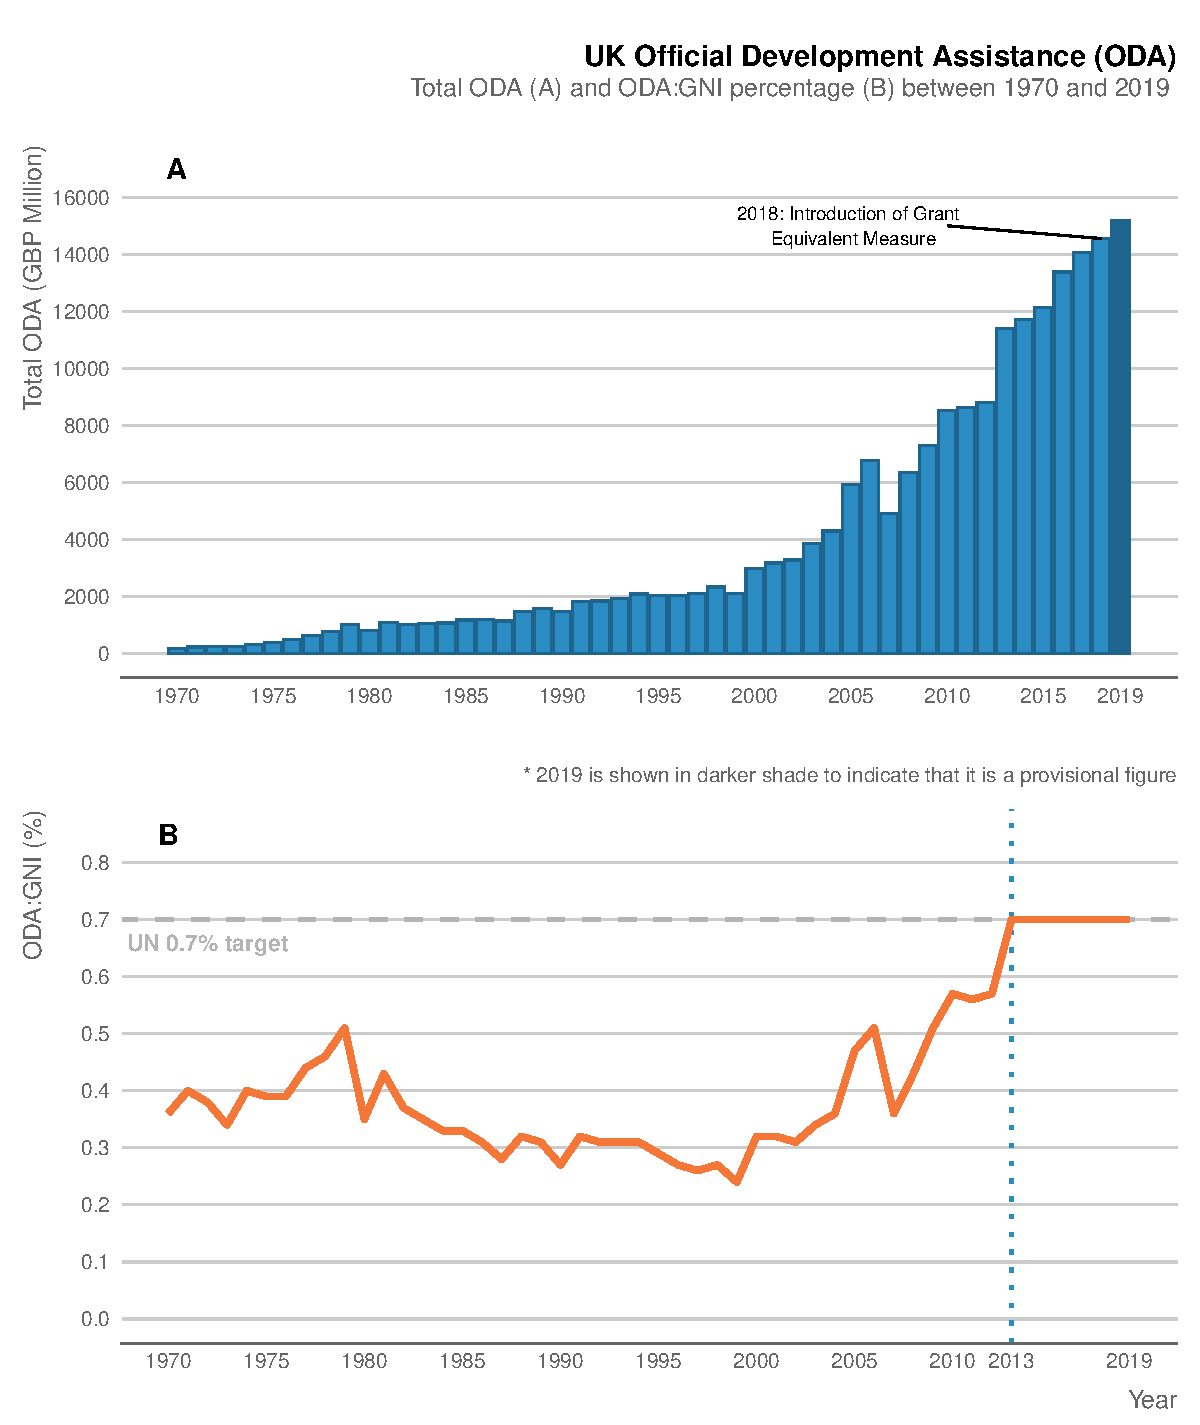
\includegraphics[width=0.9\textwidth]{figs/oda_gni_plot-1} 

\end{knitrout}
  %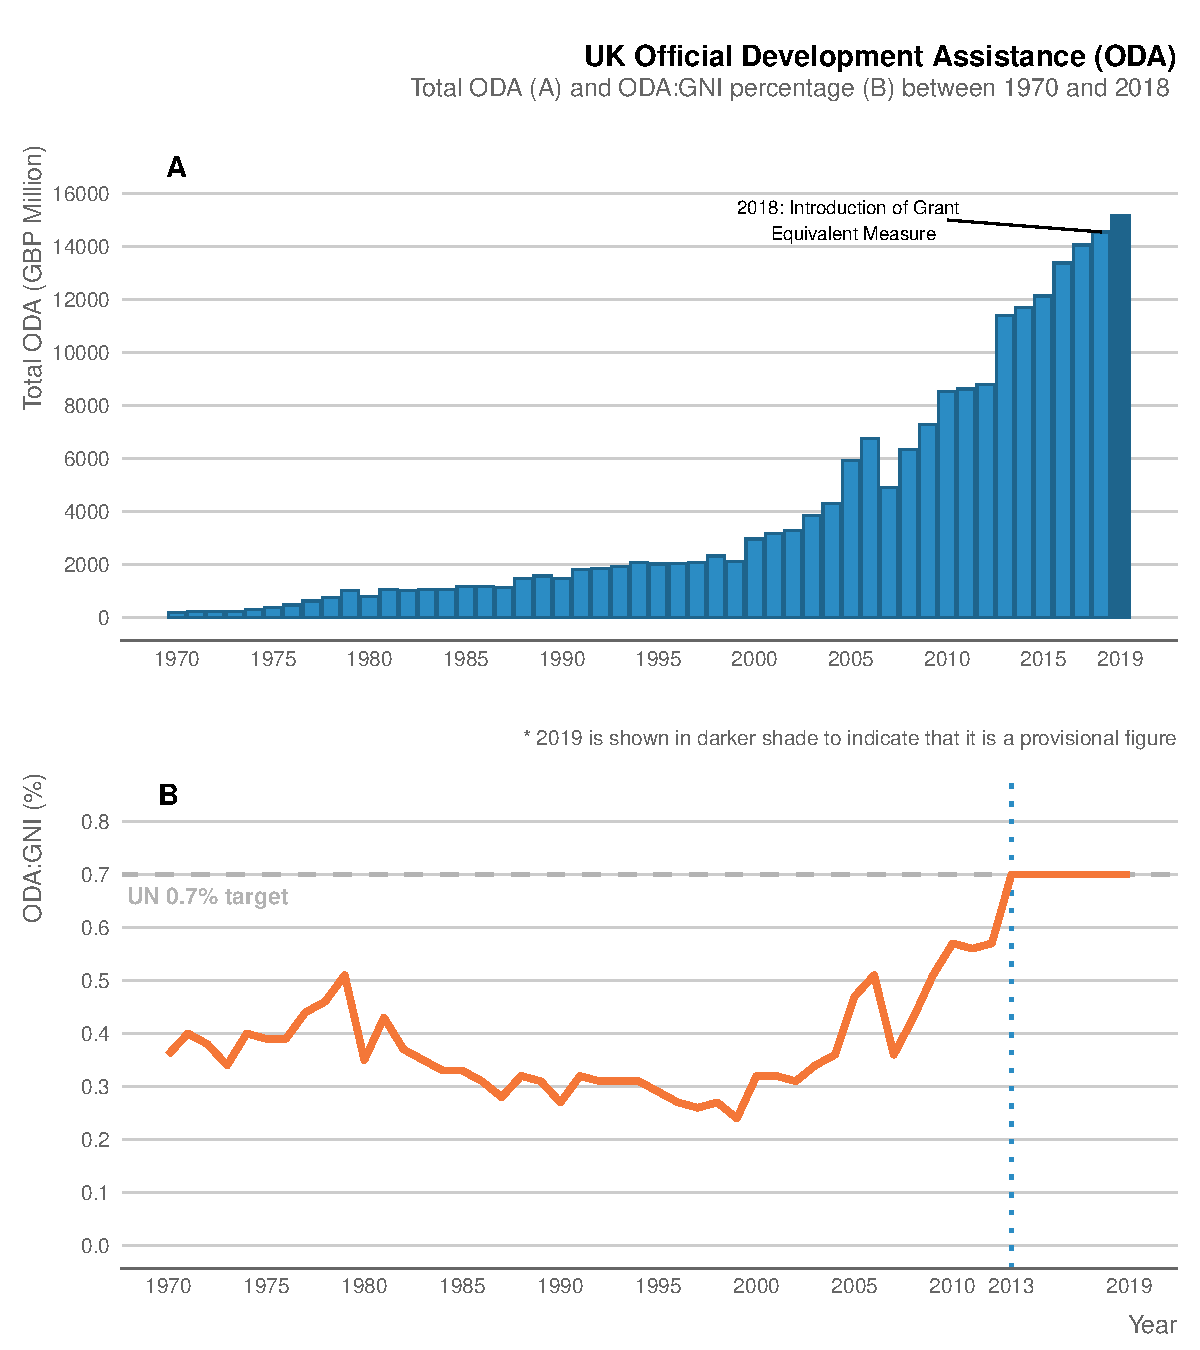
\includegraphics[width=1\textwidth]{../figs/oda_gni_plot} \hfill
  \caption{UK ODA level and ODA as a percentage of GNI between 1970 and 2019.}
  \label{fig:oda_gni_plot}
\end{figure}

For more information on UK aid spending please follow link to DFID's national statistics publication \href{https://www.gov.uk/government/statistics/statistics-on-international-development-provisional-uk-aid-spend-2019}{Statistics on International Development: UK Aid Spend 2019}. %

\section{Context}

The United Nations General Assembly agreed on an international target of 0.7\% for the ODA:GNI ratio in 1970. %
The UK government first made a commitment to increase total UK ODA to 0.7\% of GNI by 2013, and in 2015 the commitment was enshrined in UK law. %

\newpage

